\documentclass[a4paper,12pt]{article}
\usepackage[slovene]{babel}
\usepackage[utf8]{inputenc}
\usepackage{graphicx}
\usepackage{amsfonts}

\setlength{\parindent}{0mm}

\newcommand{\pojem}[1]{\textsc{#1}}

\newcounter{definicija}
\newenvironment{definicija}
{
       \stepcounter{definicija}
       \begin{flushleft}
       \textbf{Definicija \arabic{definicija}:}
}
{
       \hfill $\square$
       \end{flushleft}
}

\begin{document}
%%%%%%%%%%%%%%%%%%%%%%%%%%%%%%%%%%%%%%%%%%%%%%%%%%%%%%%%%%%%%%%%%%%%%%%%


\begin{center}
\large{textbf{Magični kvadrati}}
\end{center}

Prirejeno iz virov:
\begin{itemize}
  \item\texttt{http://mathworld.wolfram.com/MagicSquare.html}
   \item\texttt{http://en.wikipedia.org/wiki/Magic\_square}
\end{itemize}
$$
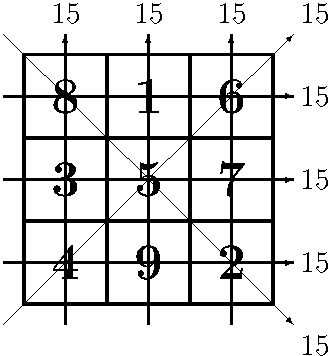
\includegraphics{slika.pdf}
$$

\tableofcontents

\newpage
%%%%%%%%%%%%%%%%%%%%%%%%%%%%%%%%%%%%%%%%%%%%%%%%%%%%%%%%%%%%%%%%%%%%%%%%

\section{Uvod}
\begin{definicija}
  \pojem{Magični kvadrat} s stranico $n$ je nabor $n^2$ različnih števil,
   ki so razvrščena v kvadratno tabelo tako, da vedno dobimo enako vsoto,
   če seštejemo vsa števila poljubne vrstice, vsa števila poljubnega
   stolpca ali vsa števila v katerikoli od glavnih diagonal.

Primer magičnega kvadrata s stranico 3 je prikazan v tabeli $1$.
\begin{table}[h]
\centering
\caption{Magični kvadrat $3\times3$}
\vspace{2mm}
\label{3x3}
\begin{tabular}{|c|c|c|}
   \hline
   8 & 1 & 6 \\ \hline
   3 & 5 & 7 \\ \hline
   4 & 9 & 2 \\ \hline
\end{tabular}
\end{table}
\end{definicija}
\begin{definicija}
   Magični kvadrat s stranico $n$ je \pojem{normalen}, če v njem nastopajo števila

$$1,2,3,\dots,n^2-1,n^2.$$

Magični kvadrat v tabeli $1$ je normalen.
\end{definicija}
%%%%%%%%%%%%%%%%%%%%%%%%%%%%%%%%%%%%%%%%%%%%%%%%%%%%%%%%%%%%%%%%%%%%%%%%

\section{Zgodovina}

\subsection{Kvadrat "`Lo Shu"'}

Kitajska literatura iz časa vsaj 2800 let pred našim štetjem govori o legendi
Lo Shu - "`zvitek reke Lo"'. V antični Kitajski je prišlo do
silne poplave. Ljudje so skušali rečnemu bogu narasle reke Lo ponuditi daritev,
da bi pomirili njegovo jezo. Iz vode se je prikazala želva z zanimivim vzorcem
na oklepu: v tabeli velikosti tri krat tri so bila predstavljena števila, tako
da je bila vsota števil v katerikoli vrstici, kateremkoli stolpcu in na obeh
glavnih diagonalah enaka: 15. To število je tudi enako številu dni v 24 ciklih
kitajskega sončnega leta. Ta vzorec so na določen način uporabljali upravljalci
reke.

Kvadrat Lo Shu
%   4 & 9 & 2 \\\hline
%   3 & 5 & 7 \\\hline
%   8 & 1 & 6 \\\hline

%%%%%%%%%%%%%%%%%%%%%%%%%%%%%%%%%%%%%%%%%%%%%%%%%%%%%%%%%%%%%%%%%%%%%%%%

Kulturna pomembnost

Magični kvadrati so fascinirali človeštvo skozi vso zgodovino. Najdemo jih
v številnih kulturah, npr. v Egiptu in Indiji, vklesane v kamen ali
kovino, uporabljane kot talismane za dolgo življensko dobo in v
izogib boleznim.

Kubera-Kolam je talna poslikava, ki se uporablja v Indiji, in je v
obliki magičnega kvadrata s stranico 3. Ta je v bistvu enak kot kvadrat
Lo Shu, vendar je vsako število povečano za 19.

Kvadrat Kubera-Kolam
%   23 & 28 & 21 \\\hline
%   22 & 24 & 26 \\\hline
%   27 & 20 & 25 \\\hline

Z magičnimi kvadrati so se ukvarjali tudi najbolj znani matematiki kot na
primer Euler, glej ??.

%%%%%%%%%%%%%%%%%%%%%%%%%%%%%%%%%%%%%%%%%%%%%%%%%%%%%%%%%%%%%%%%%%%%%%%%

Zgodnji kvadrati s stranico 4

Najzgodnejši znani magični kvadrat s stranico 4 je bil odkrit na napisu
v Khajurahu v Indiji in v Enciklopediji Bratovščine Čistosti iz enajstega
ali dvanajstega stoletja. Vrh vsega gre celo za "`panmagični kvadrat"'.

V Evropi sta morda najbolj znana naslednja magična kvadrata s stranico 4:

Magični kvadrat v litografiji Melancholia I (glej sliko ??
za izsek s kvadratom) Albrechta Durerja naj bi bil najzgodnejši magični kvadrat
v evropski umetnosti. Zelo podoben je kvadratu Yang Huija, ki je nastal na Kitajskem
približno 250 let pred Durerjevim časom.

Vsoto 34 je mogoče najti pri seštevanju števil v vsaki vrstici, vsakem stolpcu,
na vsaki diagonali, v vsakem od štirih kvadrantov, v sredinskih štirih poljih,
v štirih kotih, v štirih sosedih kotov v smeri urinega kazalca (??), v
štirih sosedih kotov v nasprotni smeri urinega kazalca (??), v dveh naborih
simetričnih parov (?? in ??), in še na nekaj drugih načinov.
Števili na sredini spodnje vrstici tvorita letnico litografije: 1514.

Durerjev magični kvadrat ??
%   16 &  3 &  2 & 13 \\\hline
%    5 & 10 & 11 &  8 \\\hline
%    9 &  6 &  7 & 12 \\\hline
%    4 & 15 & 14 &  1 \\\hline
\begin{figure}
\centering
\caption{Durerjev magični kvadrat}
\label{durer}
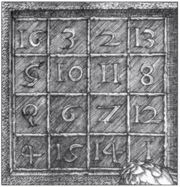
\includegraphics[scale = 1.3]{durer.jpg}
\end{figure}

Pasijonska fasada na katedrali Sagrada familia v Barceloni (glej sliko
?? za fotografijo) vsebuje magični kvadrat s stranico 4.

Pasijonska fasada, Sagrada Familia
%    1 & 14 & 14 &  4 \\\hline
%   11 &  7 &  6 &  9 \\\hline
%    8 & 10 & 10 &  5 \\\hline
%   13 &  2 &  3 & 15 \\\hline

Magični kvadrat na Sagradi Familiji

Vsota števil v vrsticah, stolpcih oziroma na diagonalah je 33 - Jezusova starost
v času pasijona. Strukturno je kvadrat podoben Durerjevemu, vendar so števila
v štirih poljih zmanjšana za 1. Posledica je, da sta števili 10 in 14 podvojeni
in zato kvadrat ni normalen.

%%%%%%%%%%%%%%%%%%%%%%%%%%%%%%%%%%%%%%%%%%%%%%%%%%%%%%%%%%%%%%%%%%%%%%%%

Osnovne lastnosti

V normalnem magičnem kvadratu s stranico ?? je vsota vseh nastopajočih
števil (glej ?? na strani ??) enaka
??, torej je vsota
števil v eni vrstici (ali stolpcu ali na eni glavni diagonali) enaka številu

??

Število ?? je znano kot magična konstanta. Preprost račun
pokaže, da je konstanti ?? analogna konstanta ?? za
magični kvadrat, v katerem so nameščena števila ??, ??, ??,
??, ??, enaka:

??

Kvadratu v tabeli ?? ustrezata konstanti ?? in ??.

Če vsako od števil v normalnem magičnem kvadratu s stranico ?? odštejemo
od ??, dobimo nov magični kvadrat, ki je prvotnemu komplementaren.

Na primer, magičnemu kvadratu Lo Shu (glej tabelo ??) priredimo
komplementarni kvadrat, prikazan v tabeli ??.

Kvadratu Lo Shu komplementarni kvadrat
%   6 & 1 & 8 \\\hline
%   7 & 5 & 3 \\\hline
%   2 & 9 & 4 \\\hline

Vidimo, da je dobljeni kvadrat moč dobiti iz kvadrata Lo Shu tudi z zasukom za
180 stopinj okrog središča, kvadrat iz tabele ?? pa je mogoče dobiti
iz kvadrata Lo Shu z zrcaljenjem preko sredinske vodoravne črte.

Število različnih normalnih magičnih kvadratov

   Pravimo, da sta dva magična kvadrata različna, če enega ni mogoče dobiti
   iz drugega s pomočjo zasukov oziroma zrcaljenj.

Števila različnih normalnih magičnih kvadratov se nahajajo v tabeli ??.

Vse normalne magične kvadrate s stranico 4 je oštevilčil Frenicle de Bessy
leta 1693, glej ??, in jih je moč najti v knjigi ??
iz leta 1982. Število normalnih kvadratov s stranico 5 je izračunal
R. Schroeppel leta 1973 (glej Gardner ??).

Natančno število vseh različnih normalnih magičnih kvadratov s stranico 6 ni znano.
Avtorja navedenega približka sta Pinn in Wieczerkowski (glej ??), ki
sta za oceno uporabila simulacijo Monte Carlo in metode statistične mehanike.

%%%%%%%%%%%%%%%%%%%%%%%%%%%%%%%%%%%%%%%%%%%%%%%%%%%%%%%%%%%%%%%%%%%%%%%%

Primeri

V tabelah ??, ?? in ?? so prikazani
magični kvadrati velikosti 5, 6, in 9.

Magični kvadrat s stranico 5
%   17 & 24 &  1 &  8 & 15 \\\hline
%   23 &  5 &  7 & 14 & 16 \\\hline
%    4 &  6 & 13 & 20 & 22 \\\hline
%   10 & 12 & 19 & 21 &  3 \\\hline
%   11 & 18 & 25 &  2 &  9 \\\hline

Magični kvadrat s stranico 6
%    6 & 32 &  3 & 34 & 35 &  1 \\\hline
%    7 & 11 & 27 & 28 &  8 & 30 \\\hline
%   19 & 14 & 16 & 15 & 23 & 24 \\\hline
%   18 & 20 & 22 & 21 & 17 & 13 \\\hline
%   25 & 29 & 10 &  9 & 26 & 12 \\\hline
%   36 &  5 & 33 &  4 &  2 & 31 \\\hline

Magični kvadrat s stranico 9
%   47 & 58 & 69 & 80 &  1 & 12 & 23 & 34 & 45 \\\hline
%   57 & 68 & 79 &  9 & 11 & 22 & 33 & 44 & 46 \\\hline
%   67 & 78 &  8 & 10 & 21 & 32 & 43 & 54 & 56 \\\hline
%   77 &  7 & 18 & 20 & 31 & 42 & 53 & 55 & 66 \\\hline
%    6 & 17 & 19 & 30 & 41 & 52 & 63 & 65 & 76 \\\hline
%   16 & 27 & 29 & 40 & 51 & 62 & 64 & 75 &  5 \\\hline
%   26 & 28 & 39 & 50 & 61 & 72 & 74 &  4 & 15 \\\hline
%   36 & 38 & 49 & 60 & 71 & 73 &  3 & 14 & 25 \\\hline
%   37 & 48 & 59 & 70 & 81 &  2 & 13 & 24 & 35 \\\hline

%%%%%%%%%%%%%%%%%%%%%%%%%%%%%%%%%%%%%%%%%%%%%%%%%%%%%%%%%%%%%%%%%%%%%%%%

za več informacij glej \cite{bessy}

\begin{thebibliography}{99}
\bibitem{berle}
E. R. Berlekamp, J. H. Conway, R. K. Guy:
Winning Ways for Your Mathematical Plays,
Vol. 2: Games in Particular, London: Academic Press, 1982.
\bibitem{bessy}
B. Frenicle de Bessy:
Des quarrez ou tables magiques. Avec table generale des quarrez magiques de quatre de costé.
Divers Ouvrages de Mathematique et de Physique, par Messieurs de l'Academie Royale des Sciences (Ed. P. de la Hire).
Paris: De l'imprimerie Royale par Jean Anisson, 423-507, 1693.
Ponatis: Mem. de l'Acad. Roy. des Sciences 5 (1666-1699), 209-354, 1729.
\bibitem{euler}
L. Euler:
De quadratis magicis,
Commentationes arithmeticae 2 (1849), 593--602.
Ponatis: L. Euler: Opera Omnia, Series 1: Opera mathematica, Vol. 7, Birkhauser, 1992.
\bibitem{gardner}
M. Gardner:
Mathematical Games,
Scientific American 234 (1976), 118--122.
\bibitem{pinn}
K. Pinn, C. Wieczerkowski:
Number of Magic Squares from Parallel Tempering Monte Carlo,
Int. J. Mod. Phys. C 9 (1998), 541--547.
\end{thebibliography}
%%%%%%%%%%%%%%%%%%%%%%%%%%%%%%%%%%%%%%%%%%%%%%%%%%%%%%%%%%%%%%%%%%%%%%%%

\end{document}